\subsubsection{IT}
Le département de l'IT est le gardian principal de tout le tâches IT commun comme:
\begin{itemize}
  \item La gestion des environnements virtuels. (cloud ou serveur physique).
  \item La gestion de l'automatisation de processus de CI interne.
  \item La gestion des licences des applications payent (OS, applications).
  \item La gestion des appareils, périphériques, les ordinateurs portables,
  \item L'architectures, méthodologies et règles régissant l'utilisation et le stockage des données.
  \item L'administration de systèmes: la configuration, gestion, entretien et dépanne des environnement
  informatique multi-utilisateur (cloud ou physique).
  \item  La gestion ou l'aide aux autres département avec la culture et pratiques DevOps.
\end{itemize}

Aussi, l'équipe d'IT de Bonitasoft gère d'autres projets comme:
\begin{itemize}
  \item Salesforce: depuis la création des use cases jusqu'à la mise en production en garantissant la gouvernance du système avec une approche DevOps.
  \item BCD: c'est une solution fournit pour utiliser les bonnes pratiques DevOps pour la livraison continue (CI) d'une application Bonita.
\end{itemize}

L'équipe est composée de quatre personnes, dont l'une est moi.

\begin{figure}[h]
  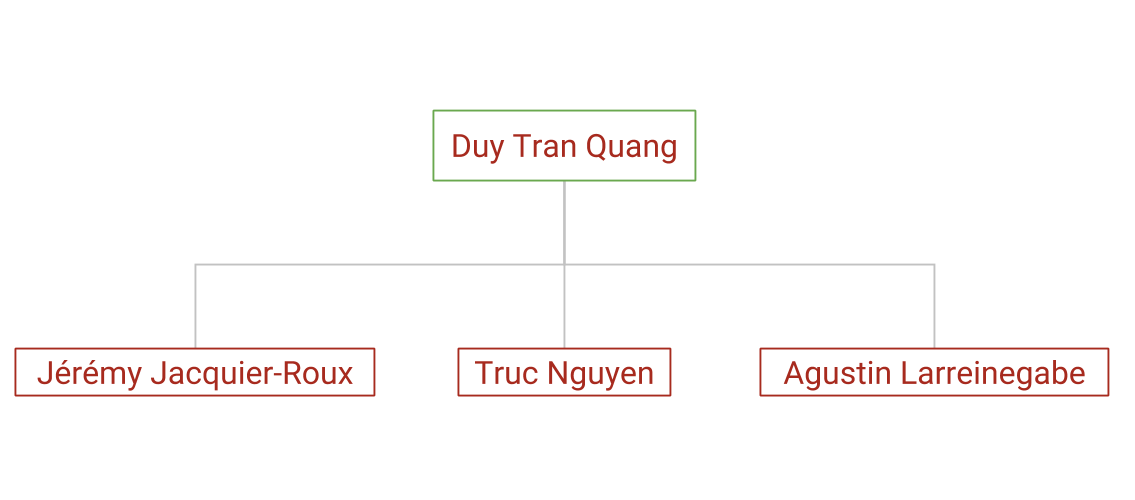
\includegraphics[width=\textwidth,keepaspectratio]{it_team.png}
   \caption{Organigramme.}
   \label{figure:organigrame}
\end{figure}
